\documentclass[12pt]{article}
\usepackage[paper=letterpaper,margin=1.5cm]{geometry}
\usepackage{amsmath,amssymb,amsfonts}
\usepackage{newtxtext, newtxmath}
\usepackage{enumitem}
\usepackage{titling}
\usepackage[colorlinks=true]{hyperref}

\usepackage{listings}
\usepackage[font=small,labelfont=bf]{caption} % Required for specifying captions to tables and figures

\usepackage{graphicx} % Required for the inclusion of images
\graphicspath{{./images/}} % Specifies the directory where pictures are stored

\setlength{\droptitle}{-6em}

\begin{document}

\center
Aprendizagem 2024\\
Homework I -- Group 016\\
(ist1106022, ist1106720)\vskip 1cm

\large{\textbf{Part I}: Pen and paper}\normalsize

\begin{enumerate}[leftmargin=\labelsep, label=\textbf{\arabic*.)}]
    \item \begin{itemize}
              \item Hamming Distance Values \\
                    \vspace{0.5em}
                    \begin{minipage}{1\textwidth}
                        \begin{center}
                            \[\begin{array}{|c|c|c|c|c|c|c|c|c|}
                                    \hline
                                    d(x_i, x_j) & x_1 & x_2 & x_3 & x_4 & x_5 & x_6 & x_7 & x_8 \\
                                    \hline
                                    x_1         & -   & 2   & 1   & 0   & 1   & 1   & 1   & 2   \\
                                    x_2         & 2   & -   & 1   & 2   & 1   & 1   & 1   & 0   \\
                                    x_3         & 1   & 1   & -   & 1   & 2   & 2   & 0   & 1   \\
                                    x_4         & 0   & 2   & 1   & -   & 1   & 1   & 1   & 2   \\
                                    x_5         & 1   & 1   & 2   & 1   & -   & 0   & 2   & 1   \\
                                    x_6         & 1   & 1   & 2   & 1   & 0   & -   & 2   & 1   \\
                                    x_7         & 1   & 1   & 0   & 1   & 2   & 2   & -   & 1   \\
                                    x_8         & 2   & 0   & 1   & 2   & 1   & 1   & 1   & -   \\
                                    \hline
                                \end{array}\]
                        \end{center}
                    \end{minipage}

              \item Nearest Neighbors for each Observation

                    \begin{itemize}
                        \item \( x_1 \rightarrow x_3\text{(P)}, x_4\text{(P)}, x_5\text{(N)}, x_6\text{(N)}, x_7\text{(N)} \)
                        \item \( x_2 \rightarrow x_3\text{(P)}, x_5\text{(N)}, x_6\text{(N)}, x_7\text{(N)}, x_8\text{(N)} \)
                        \item \( x_3 \rightarrow x_1\text{(P)}, x_2\text{(P)}, x_4\text{(P)}, x_7\text{(N)}, x_8\text{(N)} \)
                        \item \( x_4 \rightarrow x_1\text{(P)}, x_3\text{(P)}, x_5\text{(N)}, x_6\text{(N)}, x_7\text{(N)} \)
                        \item \( x_5 \rightarrow x_1\text{(P)}, x_2\text{(P)}, x_4\text{(P)}, x_6\text{(N)}, x_8\text{(N)} \)
                        \item \( x_6 \rightarrow x_1\text{(P)}, x_2\text{(P)}, x_4\text{(P)}, x_5\text{(N)}, x_8\text{(N)} \)
                        \item \( x_7 \rightarrow x_1\text{(P)}, x_2\text{(P)}, x_3\text{(P)}, x_4\text{(P)}, x_8\text{(N)} \)
                        \item \( x_8 \rightarrow x_2\text{(P)}, x_3\text{(P)}, x_5\text{(N)}, x_6\text{(N)}, x_7\text{(N)} \)
                    \end{itemize}

              \item Observation Table \\
                    \vspace{0.5em}
                    \begin{minipage}{1\textwidth}
                        \[
                            \begin{array}{|c|c|c|c|c|c|c|c|c|}
                                \hline
                                obs.          & x_1 & x_2 & x_3 & x_4 & x_5 & x_6 & x_7 & x_8 \\
                                \hline
                                true          & P   & P   & P   & P   & N   & N   & N   & N   \\
                                (+) neighbors & 2   & 1   & 3   & 2   & 3   & 3   & 4   & 2   \\
                                (-) neighbors & 3   & 4   & 2   & 3   & 2   & 2   & 1   & 3   \\
                                predicted     & N   & N   & P   & N   & P   & P   & P   & N   \\
                                result        & FN  & FN  & TP  & FN  & FP  & FP  & FP  & TN  \\
                                \hline
                            \end{array}
                        \]
                    \end{minipage}

              \item Precision, Recall and F1 Calculations

                    \[
                        \text{Precision} = \frac{TP}{TP + FP} = \frac{1}{1 + 3} = 0.25
                    \]

                    \[
                        \text{Recall} = \frac{TP}{TP + FN} = \frac{1}{1 + 3} = 0.25
                    \]

                    \[
                        F1 = 2 \times \frac{\text{Precision} \times \text{Recall}}{\text{Precision} + \text{Recall}} = 2 \times \frac{0.25 \times 0.25}{0.25 + 0.25} = \frac{1}{4} = 0.25
                    \]

          \end{itemize}
    \item \begin{itemize}
              \item Improving F1-measure by three fold

                    If we consider a kNN with k = 3 and using the Hamming Distance for only the first variable (A/B), we get:

                    \vspace{1.5em}

                    \begin{minipage}{1\textwidth}
                        \begin{center}
                            \[\begin{array}{|c|c|c|c|c|c|c|c|c|}
                                    \hline
                                    d(x_i, x_j) & x_1 & x_2 & x_3 & x_4 & x_5 & x_6 & x_7 & x_8 \\
                                    \hline
                                    x_1         & -   & 1   & 0   & 0   & 1   & 1   & 0   & 1   \\
                                    x_2         & 1   & -   & 1   & 1   & 0   & 0   & 1   & 0   \\
                                    x_3         & 0   & 1   & -   & 0   & 1   & 1   & 0   & 1   \\
                                    x_4         & 0   & 1   & 0   & -   & 1   & 1   & 0   & 1   \\
                                    x_5         & 1   & 0   & 1   & 1   & -   & 0   & 1   & 0   \\
                                    x_6         & 1   & 0   & 1   & 1   & 0   & -   & 1   & 0   \\
                                    x_7         & 0   & 1   & 0   & 0   & 1   & 1   & -   & 1   \\
                                    x_8         & 1   & 0   & 1   & 1   & 0   & 0   & 1   & -   \\
                                    \hline
                                \end{array}\]
                        \end{center}
                    \end{minipage}

                    \vspace{1.5em}

                    \begin{itemize}
                        \item \( x_1 \rightarrow x_3\text{(P)}, x_4\text{(P)}, x_7\text{(N)} \)
                        \item \( x_2 \rightarrow x_5\text{(N)}, x_6\text{(N)}, x_8\text{(N)} \)
                        \item \( x_3 \rightarrow x_1\text{(P)}, x_4\text{(P)}, x_7\text{(N)} \)
                        \item \( x_4 \rightarrow x_1\text{(P)}, x_3\text{(P)}, x_7\text{(N)} \)
                        \item \( x_5 \rightarrow x_2\text{(P)}, x_6\text{(N)}, x_8\text{(N)} \)
                        \item \( x_6 \rightarrow x_2\text{(P)}, x_5\text{(N)}, x_8\text{(N)} \)
                        \item \( x_7 \rightarrow x_1\text{(P)}, x_3\text{(P)}, x_4\text{(P)} \)
                        \item \( x_8 \rightarrow x_2\text{(P)}, x_5\text{(N)}, x_6\text{(N)} \)
                    \end{itemize}

                    \vspace{1.5em}

                    \begin{minipage}{1\textwidth}
                        \[
                            \begin{array}{|c|c|c|c|c|c|c|c|c|}
                                \hline
                                obs.          & x_1 & x_2 & x_3 & x_4 & x_5 & x_6 & x_7 & x_8 \\
                                \hline
                                true          & P   & P   & P   & P   & N   & N   & N   & N   \\
                                (+) neighbors & 2   & 0   & 2   & 2   & 1   & 1   & 3   & 1   \\
                                (-) neighbors & 1   & 3   & 1   & 1   & 2   & 2   & 0   & 2   \\
                                predicted     & P   & N   & P   & P   & N   & N   & P   & N   \\
                                result        & TP  & FN  & TP  & TP  & TN  & TN  & FP  & TN  \\
                                \hline
                            \end{array}
                        \]
                    \end{minipage}

                    \vspace{1.5em}

              \item Precision, Recall and F1 Calculations

                    \[
                        \text{Precision} = \frac{TP}{TP + FP} = \frac{3}{3 + 1} = 0.75
                    \]

                    \[
                        \text{Recall} = \frac{TP}{TP + FN} = \frac{3}{3 + 1} = 0.75
                    \]

                    \[
                        F1 = 2 \times \frac{\text{Precision} \times \text{Recall}}{\text{Precision} + \text{Recall}} = 2 \times \frac{0.75 \times 0.75}{0.75 + 0.75} = \frac{3}{4} = 0.75
                    \]

          \end{itemize}
    \item \begin{itemize}
              \item Prior Probabilities

                    \[
                        \text{P(P)} = \frac{5}{9} \quad \quad \quad \text{P(N)} = \frac{4}{9}
                    \]

              \item Likelihood of $\{y_1, y_2\}$

                    Since $\{y_1\}$ and $\{y_2\}$ are dependant, we calculate the joint possibility for both positive and negative classes.

                    \[
                        P(y_1 = A, y_2 = 0 | P) = \frac{2}{5} \quad \quad \quad P(y_1 = A, y_2 = 0 | N) = 0
                    \]

                    \[
                        P(y_1 = A, y_2 = 1 | P) = \frac{1}{5} \quad \quad \quad P(y_1 = A, y_2 = 1 | N) = \frac{1}{4}
                    \]

                    \[
                        P(y_1 = B, y_2 = 0 | P) = \frac{1}{5} \quad \quad \quad P(y_1 = B, y_2 = 0 | N) = \frac{1}{2}
                    \]

                    \[
                        P(y_1 = B, y_2 = 1 | P) = \frac{1}{5} \quad \quad \quad P(y_1 = B, y_2 = 1 | N) = \frac{1}{4}
                    \]

              \item Likelihood of $\{y_3\}$

                    Assuming $\{y_3\}$ is normally distributed.

                    \[
                        \mu_P = \frac{1.1+0.8+0.5+0.9+0.8}{5} = 0.82
                    \]

                    \[
                        \sigma_P^2 = \frac{(1.1-0.82)^2 + (0.8-0.82)^2 + (0.5-0.82)^2 + (0.9-0.82)^2 + (0.8-0.82)^2}{5} = 0.0376
                    \]

                    \[
                        y_3 | P \sim N(0.82, 0.0376)
                    \]

                    \[
                        \mu_N = \frac{1+0.9+1.2+0.9}{4} = 1.0
                    \]

                    \[
                        \sigma_N^2 = \frac{(1-1.0)^2 + (0.9-1.0)^2 + (1.2-1.0)^2 + (0.9-1.0)^2}{4} = 0.015
                    \]

                    \[
                        y_3 | N \sim N(1.0, 0.015)
                    \]

              \item Bayesian Classifier

                    \[
                        P(y_3 = x | P) = \frac{1}{\sqrt{2\pi \cdot 0.0376}} e^{\frac{-1}{2} \cdot (\frac{(x - 0.82)^2}{0.0376})}
                    \]

                    \[
                        P(y_3 = x | N) = \frac{1}{\sqrt{2\pi \cdot 0.015}} e^{\frac{-1}{2} \cdot (\frac{(x - 1)^2}{0.015})}
                    \]

          \end{itemize}

    \item \begin{itemize}
              \item For (A, 1, 0.8)
                    \[
                        P(P \mid y_1 = A, y_2 = 1, y_3 = 0.8) = P(P) \cdot p(y_1 = A, y_2 = 1 \mid P) \cdot p(y_3 = 0.8 \mid P)
                    \]
                    \[
                        = \frac{5}{9} \cdot \frac{1}{5} \cdot 2.0465 = 0.227
                    \]

                    \[
                        P(N \mid y_1 = A, y_2 = 1, y_3 = 0.8) = P(N) \cdot p(y_1 = A, y_2 = 1 \mid N) \cdot p(y_3 = 0.8 \mid N)
                    \]
                    \[
                        = \frac{4}{9} \cdot \frac{1}{4} \cdot 0.8586 = 0.095
                    \]

                    Since \( P(P \mid y_1 = A, y_2 = 1, y_3 = 0.8) \) \(>\) \( P(N \mid y_1 = A, y_2 = 1, y_3 = 0.8) \), we classify (A, 1, 0.8) as Positive (P).

              \item For (B, 1, 1)
                    \[
                        P(P \mid y_1 = B, y_2 = 1, y_3 = 1) = P(P) \cdot p(y_1 = B, y_2 = 1 \mid P) \cdot p(y_3 = 1 \mid P)
                    \]
                    \[
                        = \frac{5}{9} \cdot \frac{1}{5} \cdot 1.337 = 0.1486
                    \]

                    \[
                        P(N \mid y_1 = B, y_2 = 1, y_3 = 1) = P(N) \cdot p(y_1 = B, y_2 = 1 \mid N) \cdot p(y_3 = 1 \mid N)
                    \]
                    \[
                        = \frac{4}{9} \cdot \frac{1}{4} \cdot 3.257 = 0.3619
                    \]

                    Since \( P(P \mid y_1 = B, y_2 = 1, y_3 = 1) \) \(<\) \( P(N \mid y_1 = B, y_2 = 1, y_3 = 1) \), we classify (B, 1, 1) as Negative (N).

              \item For (B, 0, 0.9)
                    \[
                        P(P \mid y_1 = B, y_2 = 0, y_3 = 0.9) = P(P) \cdot p(y_1 = B, y_2 = 0 \mid P) \cdot p(y_3 = 0.9 \mid P)
                    \]
                    \[
                        = \frac{5}{9} \cdot \frac{1}{5} \cdot 1.8895 = 0.2099
                    \]

                    \[
                        P(N \mid y_1 = B, y_2 = 0, y_3 = 0.9) = P(N) \cdot p(y_1 = B, y_2 = 0 \mid N) \cdot p(y_3 = 0.9 \mid N)
                    \]
                    \[
                        = \frac{4}{9} \cdot \frac{1}{2} \cdot 2.333 = 0.518
                    \]

                    Since \( P(P \mid y_1 = B, y_2 = 0, y_3 = 0.9) \) \(<\) \( P(N \mid y_1 = B, y_2 = 0, y_3 = 0.9) \), we classify (B, 0, 0.9) as Negative (N).
          \end{itemize}

    \item \begin{itemize}
              \item Total Terms in Classes

                    \begin{itemize}
                        \item \( Amazing \rightarrow 1\)
                        \item \( run \rightarrow 1\)
                        \item \( I \rightarrow 1\)
                        \item \( like \rightarrow 1\)
                        \item \( it \rightarrow 1\)
                    \end{itemize}

                    \[
                        N_P = 1 + 1 + 1 + 1 + 1 = 5
                    \]

                    \begin{itemize}
                        \item \( Too \rightarrow 1\)
                        \item \( tired \rightarrow 1\)
                        \item \( Bad \rightarrow 1\)
                        \item \( run \rightarrow 1\)
                    \end{itemize}

                    \[
                        N_N = 1 + 1 + 1 + 1 = 4
                    \]

                    \begin{itemize}
                        \item \( Amazing \rightarrow 1\)
                        \item \( run \rightarrow 2\)
                        \item \( I \rightarrow 1\)
                        \item \( like \rightarrow 1\)
                        \item \( it \rightarrow 1\)
                        \item \( Too \rightarrow 1\)
                        \item \( tired \rightarrow 1\)
                        \item \( Bad \rightarrow 1\)
                    \end{itemize}

                    \[
                        N_N = 8
                    \]

              \item Likelihoods Calculations

                    Using the formula:
                    \[
                        p(t_i \mid c) = \frac{freq(t_i) + 1}{N_c + V}
                    \]

                    \textbf{Positive Class (P):}

                    Term: "I":
                    \[
                        p("I" \mid P) = \frac{1 + 1}{5 + 8} = \frac{2}{13}
                    \]

                    Term: "like":
                    \[
                        p("like" \mid P) = \frac{1 + 1}{5 + 8} = \frac{2}{13}
                    \]

                    Term: "to":
                    \[
                        p("to" \mid P) = \frac{0 + 1}{5 + 8} = \frac{1}{13}
                    \]

                    Term: "run":
                    \[
                        p("run" \mid P) = \frac{1 + 1}{5 + 8} = \frac{2}{13}
                    \]

                    \textbf{Negative Class (N):}

                    Term: "I":
                    \[
                        p("I" \mid N) = \frac{0 + 1}{4 + 8} = \frac{1}{12}
                    \]

                    Term: "like":
                    \[
                        p("like" \mid N) = \frac{0 + 1}{4 + 8} = \frac{1}{12}
                    \]

                    Term: "to":
                    \[
                        p("to" \mid N) = \frac{0 + 1}{4 + 8} = \frac{1}{12}
                    \]

                    Term: "run":
                    \[
                        p("run" \mid N) = \frac{1 + 1}{4 + 8} = \frac{2}{12} = \frac{1}{6}
                    \]

              \item Classifying "I like to run"

                    \textbf{Prior Probabilities:}
                    \[
                        P(P) = P(N) = \frac{1}{2}
                    \]

                    \textbf{For Positive Class (P):}
                    \[
                        P(P \mid \text{"I  like to run"}) = P(P) \cdot p("I" \mid P) \cdot p("like" \mid P) \cdot p("to" \mid P) \cdot p("run" \mid P)
                    \]
                    \[
                        = \frac{1}{2} \cdot \frac{2}{13} \cdot \frac{2}{13} \cdot \frac{1}{13} \cdot \frac{2}{13}
                    \]
                    \[
                        = \frac{1}{2} \cdot \frac{8}{28561} = \frac{4}{28561} \approx 0.00014
                    \]

                    \textbf{For Negative Class (N):}
                    \[
                        P(N \mid \text{"I  like to run"}) = P(N) \cdot p("I" \mid N) \cdot p("like" \mid N) \cdot p("to" \mid N) \cdot p("run" \mid N)
                    \]
                    \[
                        = \frac{1}{2} \cdot \frac{1}{12} \cdot \frac{1}{12} \cdot \frac{1}{12} \cdot \frac{1}{6}
                    \]
                    \[
                        = \frac{1}{2} \cdot \frac{1}{20736} = \frac{1}{20736} \approx 0.000048
                    \]

                    \textbf{Conclusion:}
                    Since \( P(P \mid \text{"I  like to run"}) \) \(>\) \( P(N \mid \text{"I  like to run"}) \), we classify the sentence "I like to run" as Positive (P).

          \end{itemize}
\end{enumerate}
\large{\textbf{Part II}: Programming}\normalsize

\begin{enumerate}[leftmargin=\labelsep, label=\textbf{\arabic*.)}]
    \item To compare the performance of a \textit{kNN} classifier with $k=5$ and a naive Bayes classifier, a 5-fold stratified cross-validation was performed on the on a heart disease dataset:

          \begin{enumerate}[label=\textbf{\alph*.)}]
              \item For comparing accuracies of the two classifiers, a box plot was generated for each:

                    \begin{center}
                        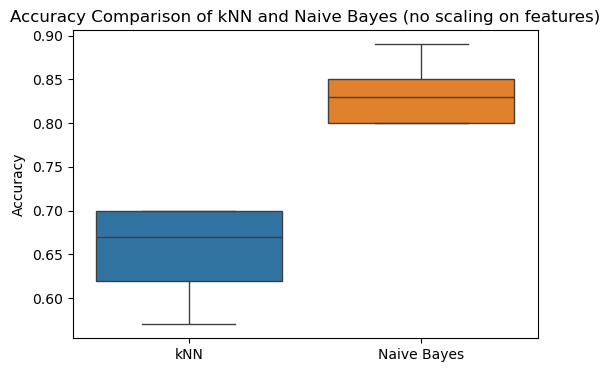
\includegraphics[width=0.8\textwidth]{boxplot_accuracies_unscaled.png}
                        \captionof{figure}{Boxplot graphs for the accuracies of the \textit{kNN} and Naive Bayes classifiers, no scaling applied on feature data}
                    \end{center}

                    The performance of the \textit{kNN} is less consistent as the box plot is wider, while the Naive Bayes classifier has a more consistent performance, as the box plot is narrower.

                    This is due to the fact that the \textit{kNN} is non-parametric and therefore is more sensitive across folds, and with non-scaled data, the distance between points is not taken into account, leading to a less accurate and more variable classification, with some classes being more dominant than others, for example.

              \item However, when choosing to scale the feature data with a Min-Max Scaler, the box plots look as follows:

                    \begin{center}
                        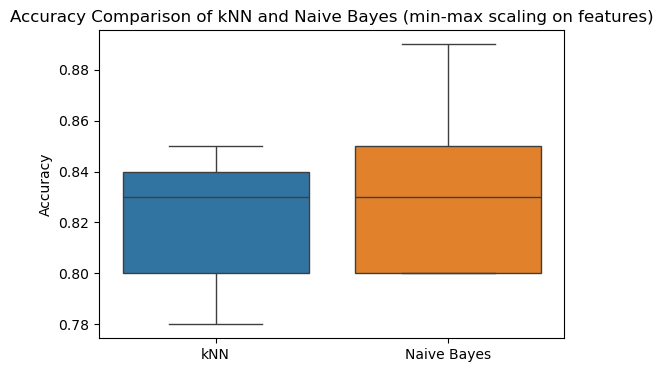
\includegraphics[width=0.8\textwidth]{boxplot_accuracies_scaled.png}
                        \captionof{figure}{Boxplot graphs for the accuracies of the \textit{kNN} and Naive Bayes classifiers, scaling data with Min-Max Scaler}
                    \end{center}

                    This happens because the \textit{kNN} classifier, when choosing to scale feature data, the distance starts becoming relevant and variability is heavily reduced, since no class imposes dominant on others, for example. This leads to a more consistent and accurate classification.

                    For \textit{Naive Bayes}, the scaling of the data does not generally affect the performance, since it is a parametric model.

              \item Perfoming a paired t-test on the accuracies of the two classifiers, using \texttt{scipy}'s method \texttt{ttest\_rel} that considers $H_0$ to be the hypothesis that the two classifiers have the same stastical significance regarding accuracy, and $H_1$ to be the hypothesis that \textit{kNN} is more accurate than Naive Bayes, the results are as follows:

                    \begin{itemize}
                        \item When not scaling feature data: $P\text{-value} = 0.998415501126768$
                              \begin{itemize}
                                  \item Considering a $1\%$ threshold, \textit{kNN} is not statistically superior than Bayes
                                  \item Considering a $5\%$ threshold, \textit{kNN} is not statistically superior than Bayes
                                  \item Considering a $10\%$ threshold, \textit{kNN} is not statistically superior than Bayes
                              \end{itemize}
                        \item When min-max scaling feature data: $P\text{-value} = 0.7532332545792753$
                              \begin{itemize}
                                  \item Considering a $1\%$ threshold, \textit{kNN} is not statistically superior than Bayes
                                  \item Considering a $5\%$ threshold, \textit{kNN} is not statistically superior than Bayes
                                  \item Considering a $10\%$ threshold, \textit{kNN} is not statistically superior than Bayes
                              \end{itemize}
                    \end{itemize}

                    We can therefore easily conclude that the hypothesis "the \textit{kNN} model is statistically superior to
                    naïve Bayes regarding accuracy" is \textbf{false / rejected}.
          \end{enumerate}
    \item To compare the performance of uniform and distance-based weights \textit{kNN} classifiers with varying amounts of neighbors (\textit{k}) used in classifications, a 80-20 train-test split was performed for each combination:

          \begin{enumerate}[label=\textbf{\alph*.)}]
              \item The following plots showcase the obtained results:

                    \begin{center}
                        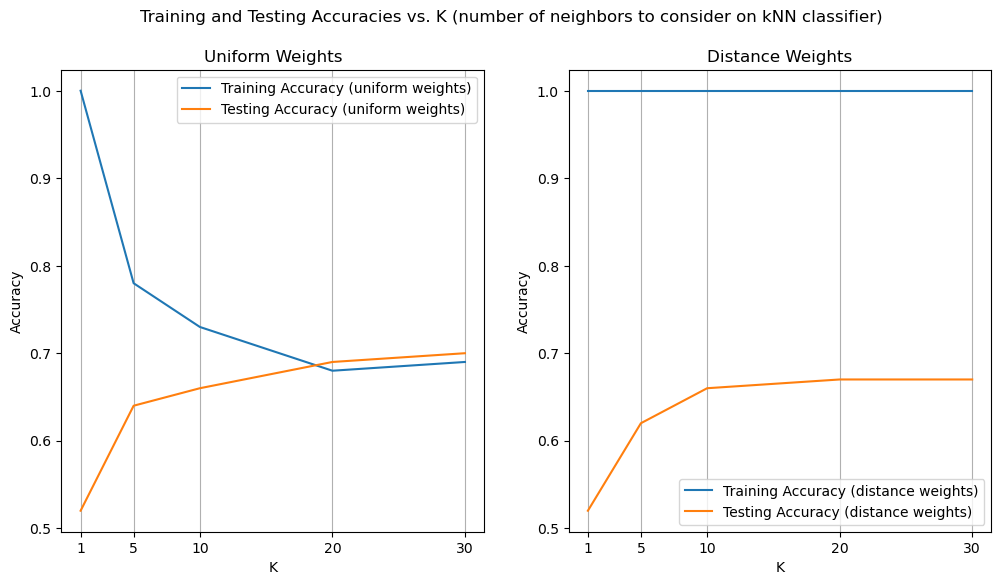
\includegraphics[width=0.8\textwidth]{kNN_accuracies.png}
                        \captionof{figure}{Accuracy plots for the \textit{kNN} classifier with uniform and distance-based weights}
                    \end{center}

              \item Generally, the bigger the value of \textit{k} on a \textit{kNN} classifier, the more accurate the predictions are, until a certain point. This point, for either uniform or distance-based weights, is when the accuracies on both training and testing data is the highest, which seems to be around $k = 20$ for this dataset.


                    In terms of generalization capabilities, the distance-based weighting system seems to be the more capable of the both, as it is capable of maintaing its accuracy on training data while also improving its accuracy on the testing data.

                    Before the suggested point, for the uniform weights, the model is overfitting on the training data.
                    Past $k=30$ both models may be at the risk of underfitting, a phenomenon not observable for the dataset at hand.

          \end{enumerate}

    \item Some properties from the dataset that may justify the shortcomings of Naive Bayes classifier on this dataset are:
          \begin{itemize}
              \item Since Naive Bayes assumes that all features are independent, it ignores the relantionships and correlation that these features may have in relation to heart disease diagnosis.
              \item The dataset has features which are not normally distributed or are not numerical, which is a violation of the Gaussian Naive Bayes conditions. Some of these features include the categorical features, such as $cp$, $fbs$, $resteg$, $exang$ and $slope$, for example.
          \end{itemize}

\end{enumerate}
\end{document}
